\chapter{Introduction}\label{chapter:introduction}

\fromsurvey{The \textit{Green Revolution} (1960s and 1970s) \citep{LLEWELLYN2018449} led to a significant increase in agricultural production \citep{evenson2003assessing} through technologies such as pesticides, fungicides, herbicides, and genetically modified crops. This development went hand in hand with the widespread establishment of monocultures and improved machinery for practically all agricultural processes. Local universities and state-owned agencies \citep{franco2001papel} played significant roles in this process. However, this revolution brought some negative aspects, such as technological dependence, deforestation, pollution, and the loss of biodiversity due to the established use of pesticides and monocultures \citep{glaeser2010green}.}

\fromsurvey{Today, as the population continues growing \citep{un_population_2024}, a further leap in agricultural productivity is required \citep{LLEWELLYN2018449}. However, achieving this leap is a greater challenge, as it is essential to mitigate the environmental impact of agribusiness. Moreover, this leap must be implemented in times of current climate problems that are already impacting agricultural productivity \citep{ortiz2021anthropogenic}. Therefore, the dream of sustainable agriculture, that is in harmony with the environment while being more productive, is more important than ever.}

\fromsurvey{In this context, \ac{RS} is a candidate tool to help accomplish this new ``greener revolution'' \citep{ahmed2024examination} as it allows monitoring whether crops are planted and harvested under optimal conditions, the use of precision agriculture \citep{liaghat2010review}, and other innovations such as the avoidance of poor crop rotation practices. For instance, precision agriculture allows agronomists to treat different regions of a field differently, e.g. applying chemicals locally rather than evenly across the plot \citep{zhang2002precision}, resulting in higher productivity while reducing environmental damage. In addition, \ac{RS} allows active monitoring of deforestation and reviewing what use or cover of land has been identified in the deforested area \citep{candra2020deforestation}. \ac{RS} can also predict agricultural productivity in different regions, allowing stakeholders to anticipate food shortages or other crises related to agricultural products \citep{quinn2010increased}.}

\fromsurvey{However, in large-scale crop monitoring, the price of expert data labeling for \ac{RS} can be a drawback \citep{ma2021multi}. The complexity increases with the heterogeneity and size of the \ac{SITS}, which may contain data such as optical, \ac{SAR}, \ac{LiDAR} and as well as thermal imagery, each with different characteristics \citep{joshi2023remote, Brandt2009} making active monitoring in near real-time by human experts infeasible (\autoref{fig:pastis_sits} shows an example of Sentinel 2 SITS labeling). \ac{ML}, especially \ac{DL}, offers a viable solution by enabling the analysis of heterogeneous data \citep{li2022deep} and scaling methods for global, near real-time monitoring. Such techniques have now replaced the traditional Shallow Learning techniques used in the past for Agricultural \ac{RS}, causing a transformation in the literature -- a change best explained through the last correlated survey of the area and the findings found through this review. These techniques can promote sustainable practices, compare patterns between regions with similar conditions, and detect or penalize deforestation, although the price of labeled datasets may still be a limitation.}

\begin{figure}[ht!]
\centering
\caption{Example of a Satellite Image Time Series (SITS) from Sentinel 2 with a labeling process.}
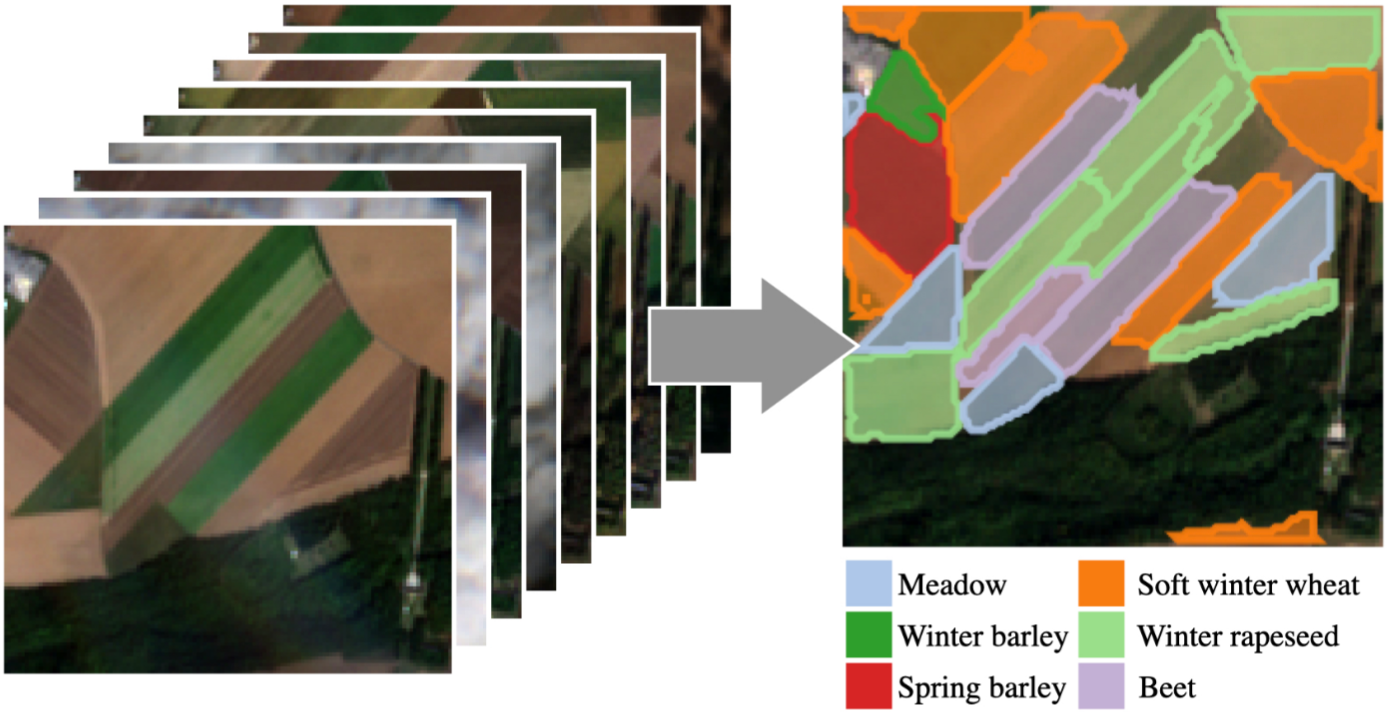
\includegraphics[width=0.75\linewidth]{figures/1_introduction/pastis-sits.png}
\fignote{Adapted from PASTIS dataset \citep{garnot2021panoptic}}
\label{fig:pastis_sits}
\end{figure}

\fromsurvey{It is important to point out that countries such as Brazil, Russia, India and China will play a crucial role in this new green revolution. These regions, in addition to their considerably large area, have significant preserved forests \citep{heino2015forest} and agricultural land \citep{pata2021linking} which makes continuous environmental monitoring essential and positions them as ideal candidates for the application of \ac{RS} techniques. However, due to limited financial resources in some emerging countries, satellite data from public missions becomes essential for supporting environmental applications in these areas.} Furthermore, it is important that the pipelines and models are also lightweight enough to run without the need for expensive hardware, since such countries may not have giant data centers available.

The reliability of predictions is a central challenge in operationalizing machine learning models for agricultural monitoring. The occurrence of incorrect classifications, or false positives generated by samples outside the training distribution, can severely compromise production estimates and the efficiency of resource allocation. It is possible that \ac{OSR} techniques such as \ac{GeMOS} \citep{vendramini2021opening} can, in addition to identifying class samples outside the training set, also possibly differentiate correct from incorrect predictions within known classes.

\fromsurvey{Moreover, the amount of unlabeled remote sensing data is considerable, as satellite images are constantly being acquired by various free-of-charge missions. This is one of the reasons why \ac{SSL} is very promising in the field of \ac{RS}, as it is able to extract patterns from unlabeled data to generate supervised signals by reconstructing masked data or data contrastivity. \ac{SSL} has became very popular in \ac{NLP} and is one of the reasons for the success of tools such as \ac{GPT} \citep{radford2018improving} and large language models such as \ac{BERT} \citep{devlin2019bert}. Thus, after pretraining a \ac{DL} model with \ac{SSL}, it is possible to train it with less labeled data, resulting in a model that is likely to be more robust and generalistic \citep{chen2020adversarial}.}

\fromsurvey{Thus, we comprehensively reviewed all publicly available labeled datasets for these applications, focusing on both agricultural and deforestation classes, including the few datasets whose study regions are emerging countries. In addition, we reviewed all satellite sensors that are publicly available to researchers and/or contain some publicly available datasets that could be useful for the research area. We also included unlabeled \ac{RS} datasets, as we have not yet found any unlabeled datasets specifically for \ac{RS} of agriculture or vegetation.}

Furthermore, it is clear that for large-scale crop monitoring, the use of paid remote sensing images becomes impractical. It is possible to imagine a pipeline divided into three main sequential stages:

\begin{enumerate}
    \item \textbf{Parcel Delineation} Identifying the geometries of agricultural plots on a given farm or in any given region.
    \item \textbf{Crop Mapping} Given the geometry of an agricultural plot, classify the species of plant grown in a given period of time.,
    \item \textbf{Crop Yielding} Given the geometry and the species of plant grown, predict what the yield (usually in tons per hectare) of that crop will be.
\end{enumerate}

In addition, there are two other applications that are more peripheral to crop monitoring, but equally important: Change Detection and Land Usage Land Cover. The first can be used to detect deforestation, which may be a step prior to planting a crop. The second can be used for more general mapping of a farm in order to detect the amount of water, for example, which can be used to refine a crop classification, since certain species require active irrigation.  

\begin{figure}[!ht]
  \caption{Diagram showing possible agricultural (a) and correlated (b) applications with Deep Learning and Remote Sensing.}
  \centering
  \begin{subfigure}[c]{0.48\columnwidth} % Reduced width
    \centering
    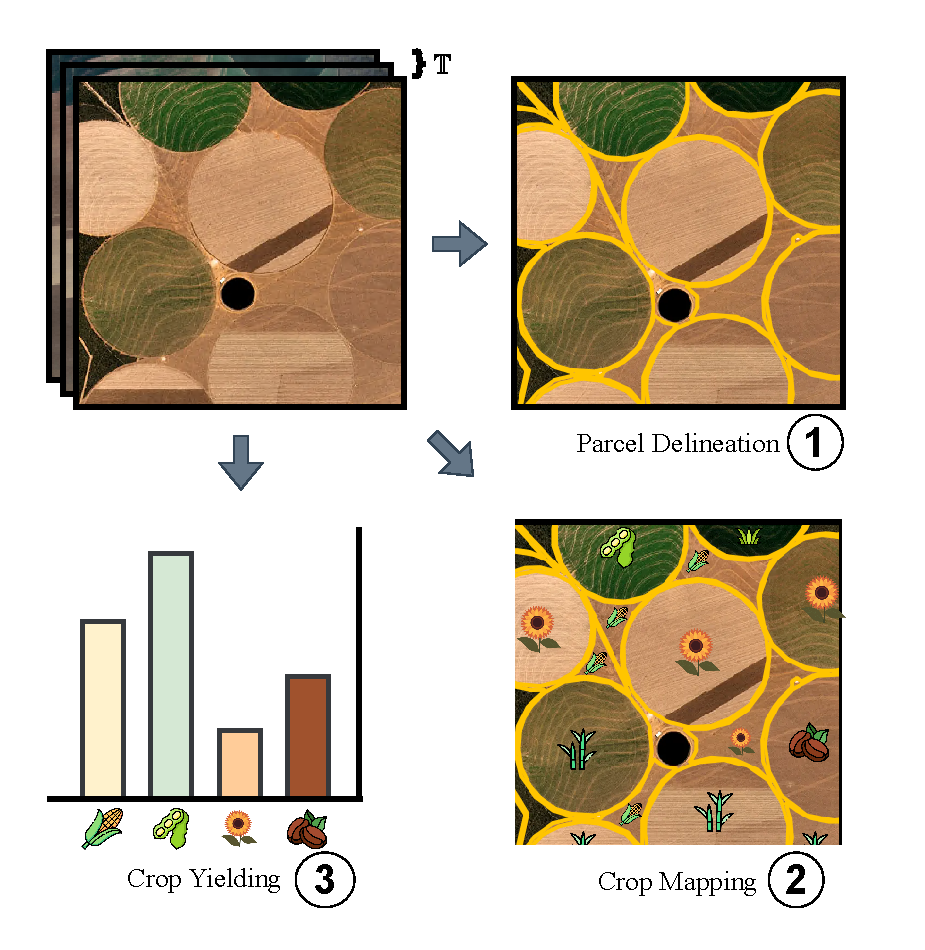
\includegraphics[width=\currprop]{figures/1_introduction/graphical_abstract_crop_new_fixed.pdf} % + 0.19
    \caption{}
    \label{fig:graphical_abstract_crop_tasks}
  \end{subfigure}
  \hfil % This provides the horizontal space
  \begin{subfigure}[c]{0.48\columnwidth} % Reduced width
    \centering
    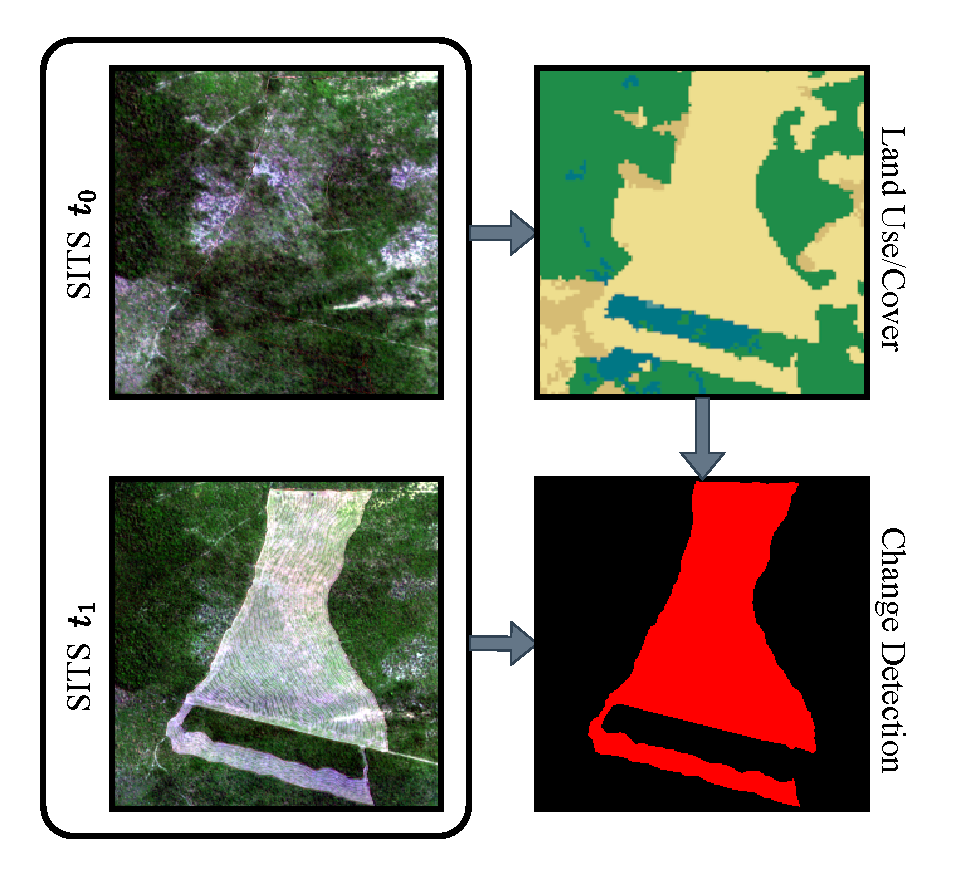
\includegraphics[clip,width=\currprop]{figures/1_introduction/graphical_abstract_lulc_cd_new.pdf}
    \caption{}
    \label{fig:graphical_abstract_lulc_cd}
  \end{subfigure}
  
  \fignote{This figure shows illustrative examples of the applications covered in this work. In Figure \ref{fig:graphical_abstract_crop_tasks}, we can observe a large-scale crop monitoring pipeline based on (1) parcel delineation, (2) crop mapping and (3) crop yielding prediction illustrated over multitemporal images. In Figure \ref{fig:graphical_abstract_lulc_cd}, two timestamps are used to compute land cover/usage and change detection. Most agricultural-related applications rely on multitemporal data across a range $\mathbb{T}$ of acquisition dates (a) or a pair $t_0$ and $t_1$ of dates (b).}
  
  \label{fig:graphical_abstract}
\end{figure}

In this study, we focus specifically on Crop Mapping, since Parcel Delineation already has foundational models that allow the application to be run without training data (see Section \ref{sec:parcel_segmentation}) and Crop Yielding has very few public datasets (see Section \ref{sec:labeled_datasets}) due to the industry's economic interest in the area, meaning that most datasets are private and focus on a subset of crop classes relevant to a geographic region. We propose a complete pipeline ranging from a rigorous strategy for building a crop mapping dataset from parcel geometries and public cropland rasters, a lightweight method for downloading samples from public mission sensors, evaluation of Shallow Learning and Deep Learning models for classification, SSL pre-training techniques, and procedures for anomaly detection.

Regarding the work developed throughout the master's program, a literature review was published at an international conference \citep{mateuzin2024} awarded with an extended version published in Computer \& Graphics \citep{daSilva2025} with a new culture classification model proposed using \ac{SSL}. In addition, part of the methodology of this dissertation work was also published as a separate paper \citep{pintodasilva2025lightweight}. Two co-supervisions of bachelor's degree final projects were conducted, one in the area of Open Set Recognition for Crop Classification and the other for super-resolution for agricultural Remote Sensing. Finally, three less related works were done, one as a result of teaching assistance in a programming course using \ac{LLM} \citep{alcantara2025assessing}, another for segmentation of 3D medical images \citep{Oliveira2025} and another about the role of data quality in remote sensing classification \citep{Correa2026rethinking}. At last, a Python library with tools for downloading and preprocessing data that can be fed to the pipeline was also published on PyPI (more details in Section \ref{sec:agl}).

\section{Research Questions}

To guide the investigation into the gaps identified in large-scale agricultural monitoring – scarcity of reliable labeled data, possible hardware limitations, use of only publicly available sensor data due to the high price of paid sensor data, and verification of correct/incorrect predictions with anomaly detection – this work is structured around six fundamental Research Questions (RQs).

\begin{enumerate}
    \item \textbf{RQ1:} To what extent can DCAI strategies - specifically, rigorous filtering of noisy public labels (such as USDA CDL or Mapbiomas) - enable the creation of crop classification datasets and improve the performance of crop classification models?
    \item \textbf{RQ2:} Do SSL pre-training strategies impact embedding generation and offer a significant advantage over supervised models when labels are scarce? If so, which strategy generates the best embeddings?
    \item \textbf{RQ3:} Is it possible to build a lightweight pipeline that achieves satisfactory performance for crop classification that can be run without expensive hardware? If so, which models are most suitable?
    \item \textbf{RQ4:} Is it possible to achieve satisfactory performance for crop classification using only public sensors?
    \item \textbf{RQ5:} Is it possible to improve confidence estimation or detect model anomalies - differ between right and wrong predictions - through generative models on embeddings, surpassing established baselines such as ConfidNet \citep{corbiere2019addressing} in the task of fault prediction?
\end{enumerate}

\section{Aims and Objectives}

The main objective of this work is to develop and validate a reliable, lightweight, data-centric pipeline for crop classification at the plot level, using public SITS, capable of distinguishing between known and unknown crops and predicting its own failures. The specific objectives are:

\begin{itemize}
    \item Analyze and curate publicly labeled agricultural datasets from large producers (US and Brazil), applying data-centric filtering techniques to mitigate label noise;
    \item Evaluate the suitability of public sensors (Sentinel-2) for capturing spectral-temporal patterns of crops.
    \item Implement and publicize a lightweight pipeline for downloading and preprocessing SITS time series of optical data from parcel geometries;
    \item Implement and compare DL/SL architectures in terms of metrics and computational cost.
    \item Investigate the impact of different SSL pre-training techniques on the quality of the generated embeddings and their transfer learning capability;
    \item Develop and validate a DCAI confidence estimation strategy based on generative model optimization (called \ac{ORDER}, based on \ac{GeMOS} \citep{vendramini2021opening}) and compare it with the ConfidNet \citep{corbiere2019addressing} baseline to detect incorrect predictions.
\end{itemize}

\section{Contributions}

To achieve the aforementioned objectives and address the research questions posed in this study, this thesis proposes a comprehensive methodology that spans from rigorous data curation and lightweight data acquisition to extensive model benchmarking and advanced anomaly detection. Specifically, the main contributions of this work to the fields of Agricultural Remote Sensing and Machine Learning are summarized as follows:

\begin{itemize}
    \item \textbf{Curation Methodology for creating parcel-level crop classification datasets:} We propose a rigorous protocol for filtering and cleaning noisy public labels based on a Cropland raster and parcel delineation, which generates a parcel-level crop classification dataset to train the models in the subsequent steps;
    \item \textbf{Lightweight SITS Download Methodology:} We develop an efficient method for downloading satellite image time series (SITS) using Google Earth Engine (GEE), optimizing the process to reduce computational costs and download time;
    \item \textbf{Evaluation of Simple vs. Complex Models:} Comparative analysis showing the effectiveness of lightweight architectures (MLPs and SL) compared to DL models, ranging from 1D CNN, LSTM, Transformer to the post-transformer MAMBA architecture;
    \item \textbf{SSL Pre-training Benchmark}: Comparative evaluation of reconstruction (MIM), contrastive (MoCo), non-contrastive (FastSiam), and hybrid (PMSN) strategies for pre-training models in agricultural SITS.
    \item \textbf{Development of the \ac{ORDER} Method:} We propose \ac{ORDER}, a hyperparameter search strategy applied to the \ac{GeMOS} \cite{vendramini2021opening} framework. Unlike standard anomaly detection, \ac{ORDER} maximizes the Area Under the Curve (AUC) by specifically considering the separability between correctly and incorrectly classified samples for each class;
    \item \textbf{Confidence Estimation Benchmarking:} We perform a comparative evaluation of model reliability using ConfidNet \citep{corbiere2019addressing} as a baseline against the proposed \ac{ORDER} approach, focusing on maximizing failure prediction;
    \item \textbf{Open Source Tools:} Publication of the time series download method, among other additions, in the AgriGEE.lite library to facilitate research in the area.
\end{itemize}

\section{Thesis Outline}

The remainder of this thesis is organized as follows. Chapter \ref{chapter:theoretical_background} introduces the necessary theoretical background, addressing concepts of Agricultural Remote Sensing, observation satellites, and Machine Learning principles, from \ac{SL} to \ac{DL}, also detailing \ac{SSL}. Next, Chapter \ref{chapter:related_works} presents a review of related works and a taxonomy of the area, covering applications directly related to agriculture -- Parcel Delineation, Crop Mapping, and Crop Yielding -- and indirect applications -- \ac{LULC} and Change Detection.

The Chapter \ref{chapter:meth_data} describes data acquisition and datasets made from \ac{SITS}, detailing the pipeline for creating parcel-level datasets for the regions of Texas, California, and Brazil, as well as the lightweight download strategy implemented in the AgriGEE.lite library. Subsequently, Chapter \ref{chapter:meth_model} explores the learning methods used in the study, including \ac{SL}, \ac{DL}, and \ac{SSL}, as well as techniques aimed at anomaly detection.

The experimental setup is defined in Chapter \ref{chapter:exp_setup}, which lists the evaluation metrics employed, hardware used, hyperparameter search space, tests performed, and data scenarios considered. Finally, Chapter \ref{chapter:results} reports the quantitative results obtained, both from pre-training and generated embeddings, as well as from fine-tuning. It also discusses the findings in the context of the current literature and technological changes in the field. At last, Chapter \ref{chapter:conclusion} presents the concluding remarks of this work, summarizing the contributions and answering the research questions.